%------------------------------------------------
\subsection{Particle Flow Network (Supervised)}
\label{subsec:supervised}
\subsubsection{Architecture Fundamentals}

A Particle Flow Network (PFN)~\cite{pfn} architecture is selected for two reasons: \textit{permutation invariant input modeling} to best describe the events consisting of an unordered set of particles, and a \textit{low-level input modeling} using tracks to take advantage of the available high-dimensional information to best exploit available correlations within the event. Permutation invariant input modeling is an architecture priority as ordered input modeling has been observed to bias the performance of low-level modeling tools as in \cite{vrnn}. Low-level input modeling is an architecture priority to capture the intricacies of dark QCD showers with may not express themselves in higher level variables, as explored in \cite{darkqcd}. A comparison to a high-level \textit{boosted decision tree} (BDT) is available in Appendix~\ref{app:bdtvspfn}.

The PFN is used to model input events as an unordered set of tracks. Given the inherently unordered and variable-length nature of particles in an event, this choice of modeling as a \textit{set} can enable the model to better learn the salient features of the dataset that enable a signal-to-background classification. Constructing the PFN involves the creation of new basis variables $\Phi$ for each particle in the event. Permutation invariance is enforced by summing over the $\Phi$ basis for every particle in the event to create a new permutation invariant latent space basis $\mathcal{O}$. Finally the classifier $F$ is a function of the sum over this new basis. The creation of the latent space basis $\mathcal{O}$ from $M$ particles $\vec{p}$ with $d$ features each can be expressed as:

\begin{equation}
  \mathcal{O}(\{\vec{p_1},...,\vec{p_M}\}) = \sum_{i=1}^M \Phi_i(\vec{p_i})
  \label{eq:pfn}
\end{equation}

where $\Phi : \mathbb{R}^d \rightarrow \mathbb{R}^l$ is a per particle mapping, with $l$ being the dimension of the new basis $\mathcal{O}$. Figure~\ref{fig:pfn_paper} gives a graphical representation of the use of summation in the PFN over per-particle information to create a permutation-invariant event representation. \par
\begin{figure}[!htbp]
\centering
   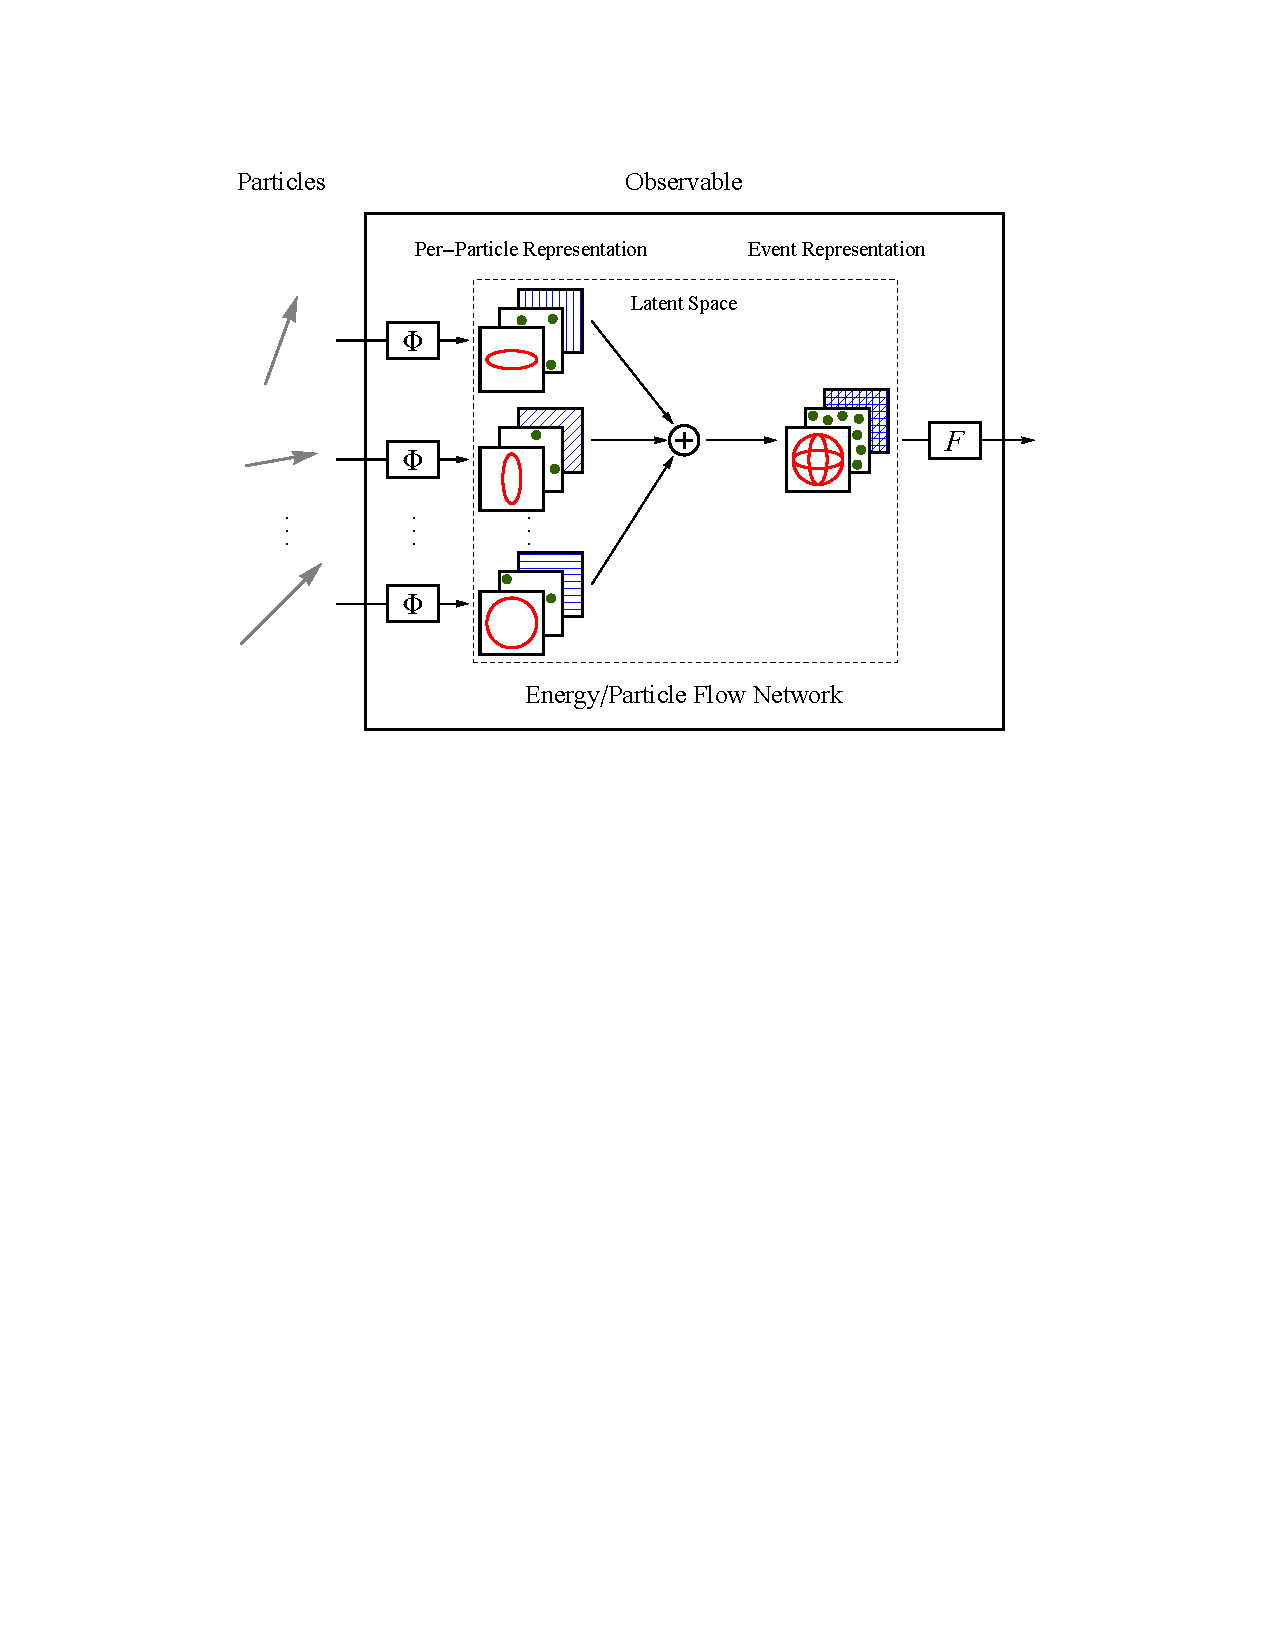
\includegraphics[width=0.7\textwidth]{figures/ml/pfn_paper}
    \caption{The Energy/Particle Flow Network concept, from Ref.~\cite{pfn}.
    \label{fig:pfn_paper}}
\end{figure}

Figure~\ref{fig:pfn_arch} provides an annotated diagram of the PFN architecture as used in this analysis. 
\begin{figure}[!htbp]
\centering
   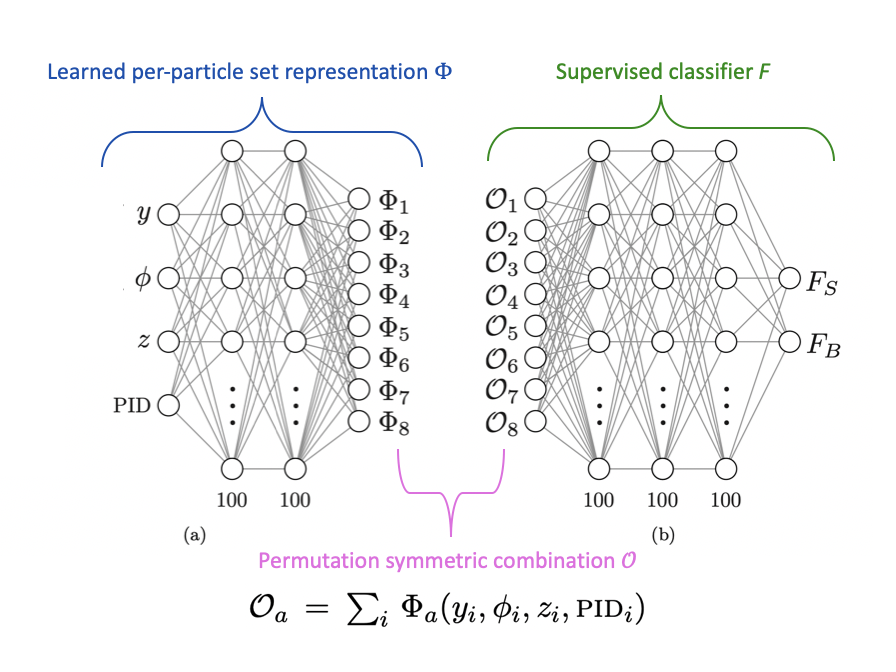
\includegraphics[width=0.9\textwidth]{figures/ml/pfn_arch}
    \caption{An annotated diagram of the PFN architecture. $y$ and $\phi$ represent geometric information for the input particles, $z$ represents energy information, and PID encompasses any other particle ID information in the input.
        \label{fig:pfn_arch}}
\end{figure}

%--------------------
\subsubsection{Input Modeling, Scaling, and Rotation}
\label{sec:input_model}
In this implementation, the particle input information comes from all tracks associated to the leading and subleading jets. The track association method is Ghost association, as discussed in Section~\ref{sec:ghost}. A single jet tagger strategy was also considered, but utilizing tracks from both leading jets creates a complete low-level picture of the event, which both focuses on the objects most likely to be associated to the decay of the dark quark (as will be justified in Chapter~\ref{ch:analysis}) and the relationship between those objects. If we consider the dijet topology of semi-visible jets as illustrated in Figure~\ref{fig:svj_pic}, the advantage of modeling both leading jets simultaneously becomes clear. In the semi-visible jet model presented in \cite{darkqcd}, \met in the event is expected to arise due to an imbalance in the number of visible tracks of the two jets associated to the dark quark decay.\par

\begin{figure}[!htbp]
\centering
   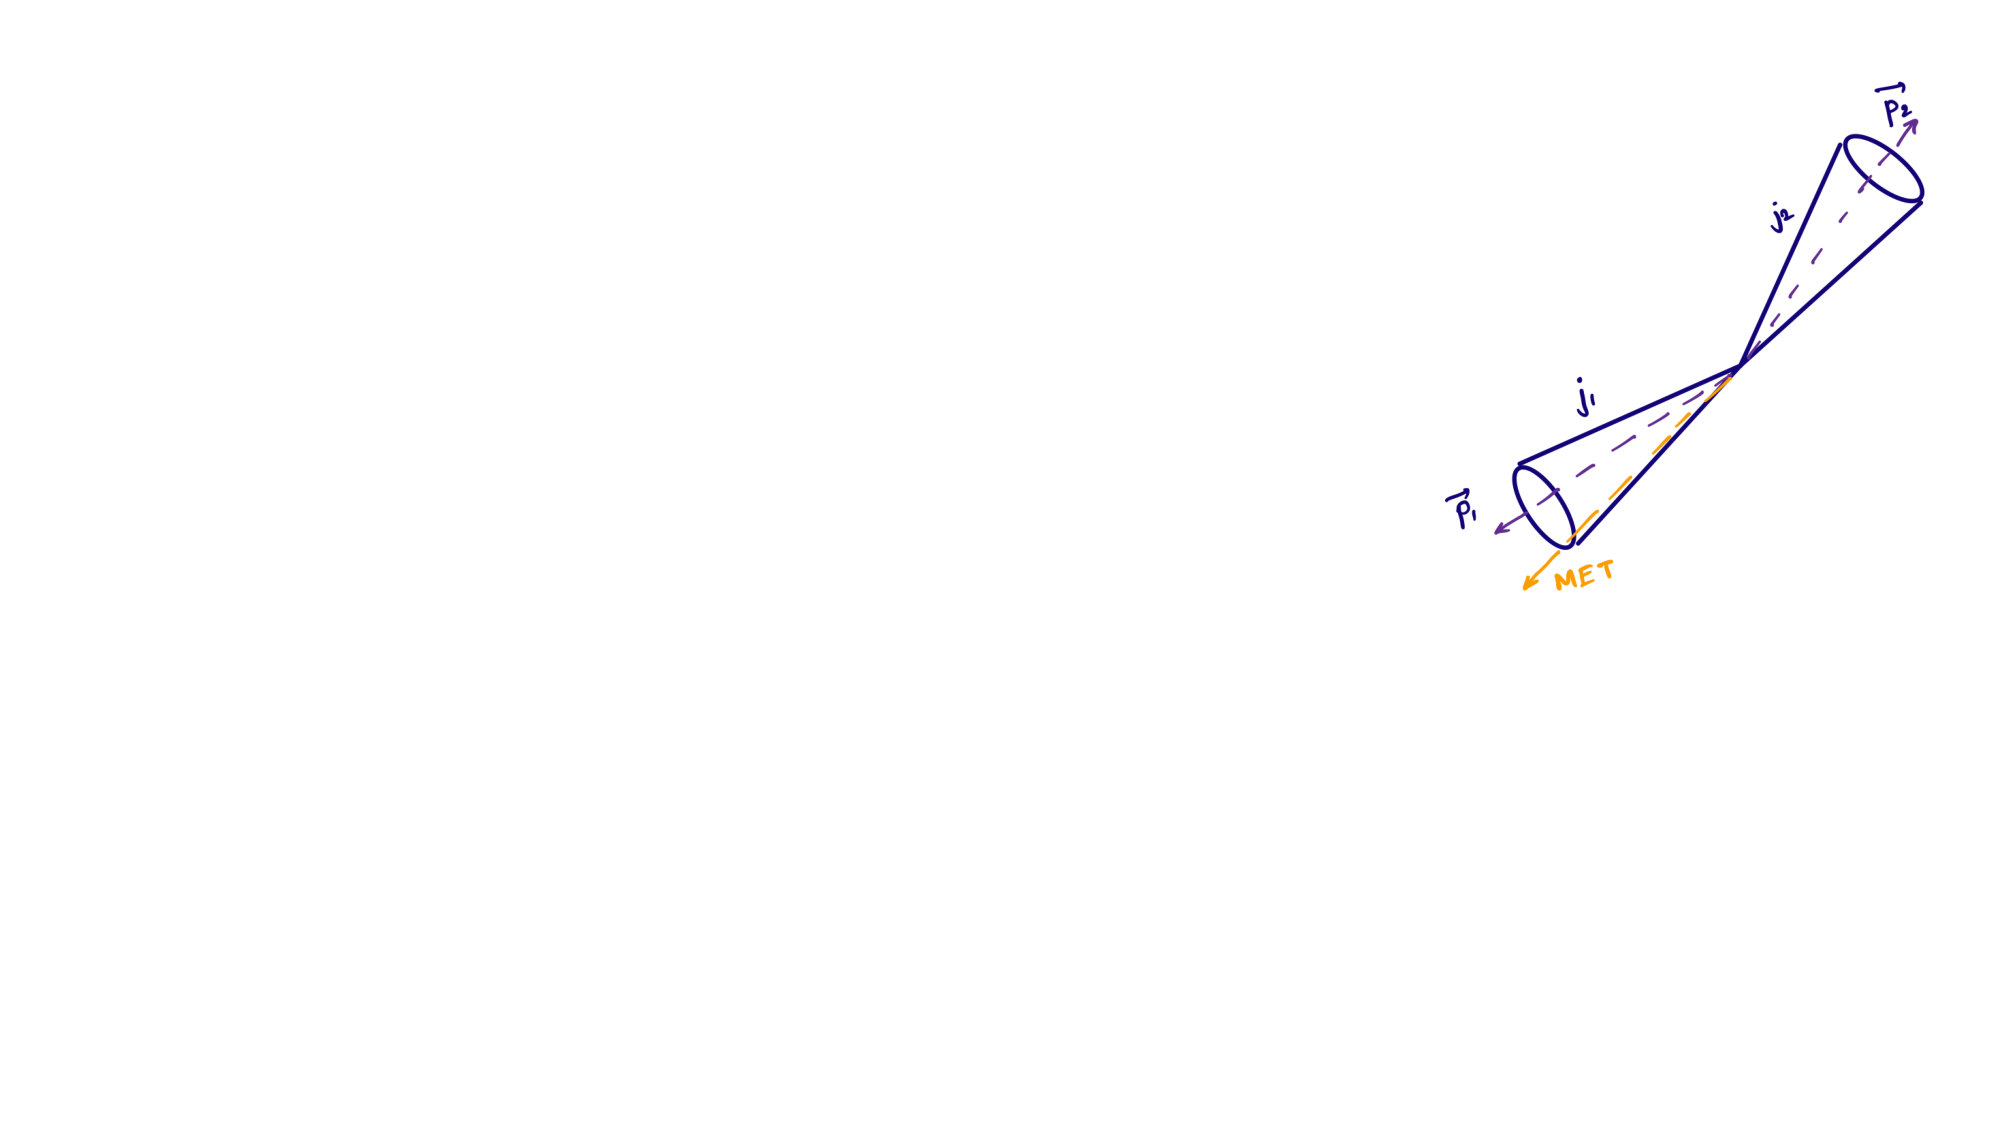
\includegraphics[width=0.4\textwidth]{figures/ml/dijet_topology}
    \caption{A illustration of the expected dijet behavior of semi-visible jets, where one jet is closely aligned with \met.
        \label{fig:svj_pic}}
\end{figure}

Each track is described using six variables: the four-vector of the track (\pt, $\eta$, $\phi$, E), and the track displacement parameters $d_0$ and $z_0$, where $d_0$ measures displacement in the radial direction from the beamline and $z_0$ measures displacement along the beamline from the primary interaction point. Figure~\ref{fig:trackcoordinates} illustrates these coordinates. Up to 80 tracks per jet are allowed, which is a threshold chosen to generally include all the tracks in the jet, which leads to maximal performance. Figure~\ref{fig:ntracks} shows the track multiplicity in the leading and subleading jet for the signal and background samples used in training. \par

\begin{figure}[!htbp]
\centering
   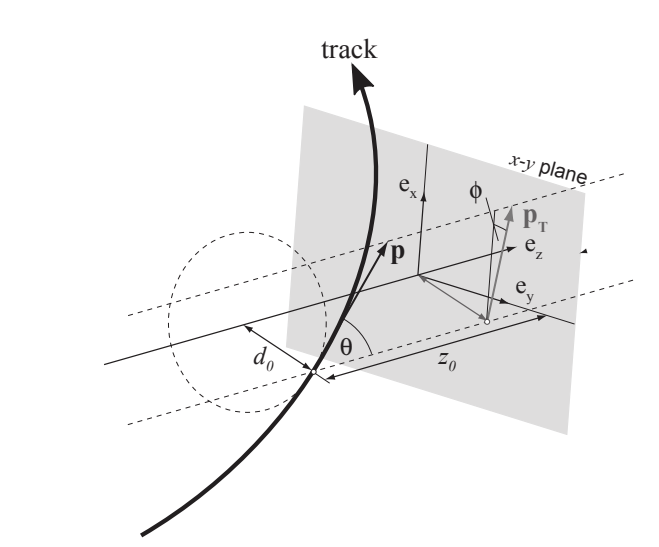
\includegraphics[width=0.4\textwidth]{figures/ml/trackcoordinates}
    \caption{Illustration of track coordinates $d_0$ and $z_0$.
    \label{fig:trackcoordinates}}
\end{figure}

\begin{figure}[!htbp]
\centering
   \includegraphics[width=0.95\textwidth]{figures/ml/ntracks}
    \caption{Distributions of the track multiplicity in the leading and subleading jets, comparing signal and background PFN training samples.
    \label{fig:ntracks}}
\end{figure}

These tracks (up to 160 total) are the input to the PFN. Referencing Equation~\ref{eq:pfn}, this corresponds to $M = 160$ and $d = 6$. The two leading jets and their associated tracks are rotated so that the center of the system is aligned with $(\eta,\phi) = (0,0)$. Each track is normalized to its relative fraction of the total dijet system energy and transverse momentum- this enforces agnosticism to the total energy and transverse momentum of the event. The rotation and scaling are motivated by the procedures described in~\cite{pfn} to improve the optimality of the PFN  learning. Figure~\ref{fig:jet_rotate} illustrates the rotation process.

\begin{figure}[!htbp]
\centering
   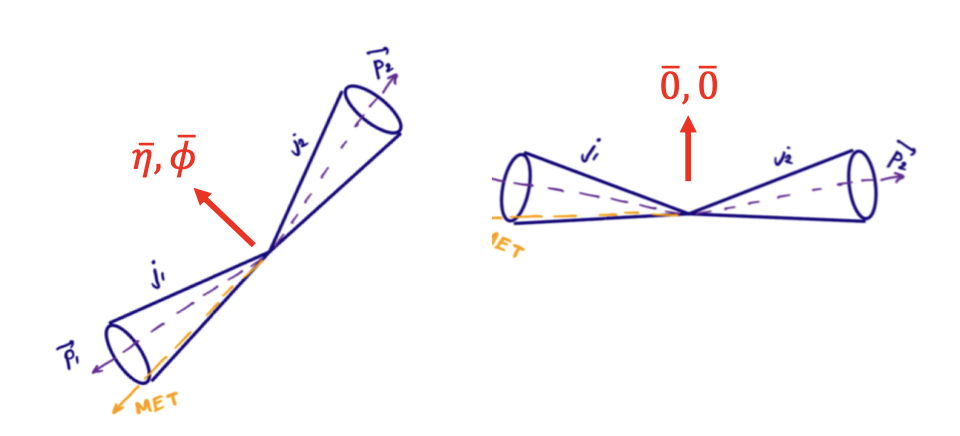
\includegraphics[width=0.65\textwidth]{figures/ml/jet_rotate}
    \caption{A diagram demonstrating how the two jet system is rotated in $(\phi,\eta)$.
    \label{fig:jet_rotate}}
\end{figure}

Finally, each of the 6 track variables is scaled so that its range is [0,1]. This is a common preprocessing step that ensures the input data is bounded over a similar range, so that arbitrarily large values don't develop an outsized impact on the model. Figure~\ref{fig:pfn_bkgsig_input} show each of 6 track variables before and after scaling and rotation have been applied, demonstrating the impact of these procedures, as well as the track level similarities differences between the background SM QCD processes and the signal SVJ processes. Figure~\ref{fig:pfn_datamc_input} illustrates that the data is well modeled by the MC at track level.

\begin{figure}[!htbp]
\centering
   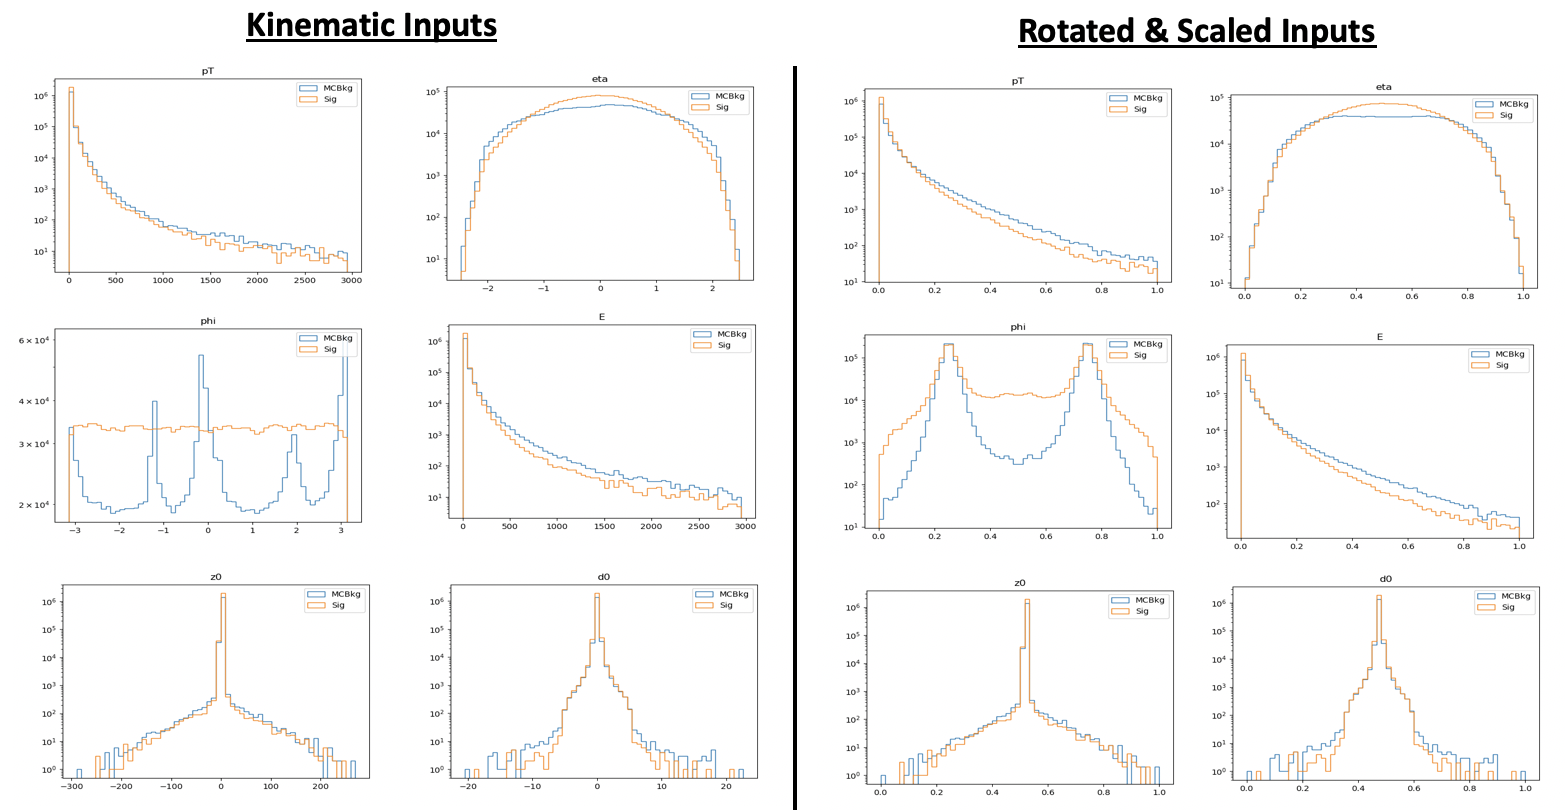
\includegraphics[width=\textwidth]{figures/ml/pfn_bkgsig_input}
    \caption{The 6 PFN track variables in background MC and signal MC. There are some differences between signal and background, but the track kinematics are largely similar. 
     \label{fig:pfn_bkgsig_input}}
\end{figure}

\begin{figure}[!htbp]
\centering
   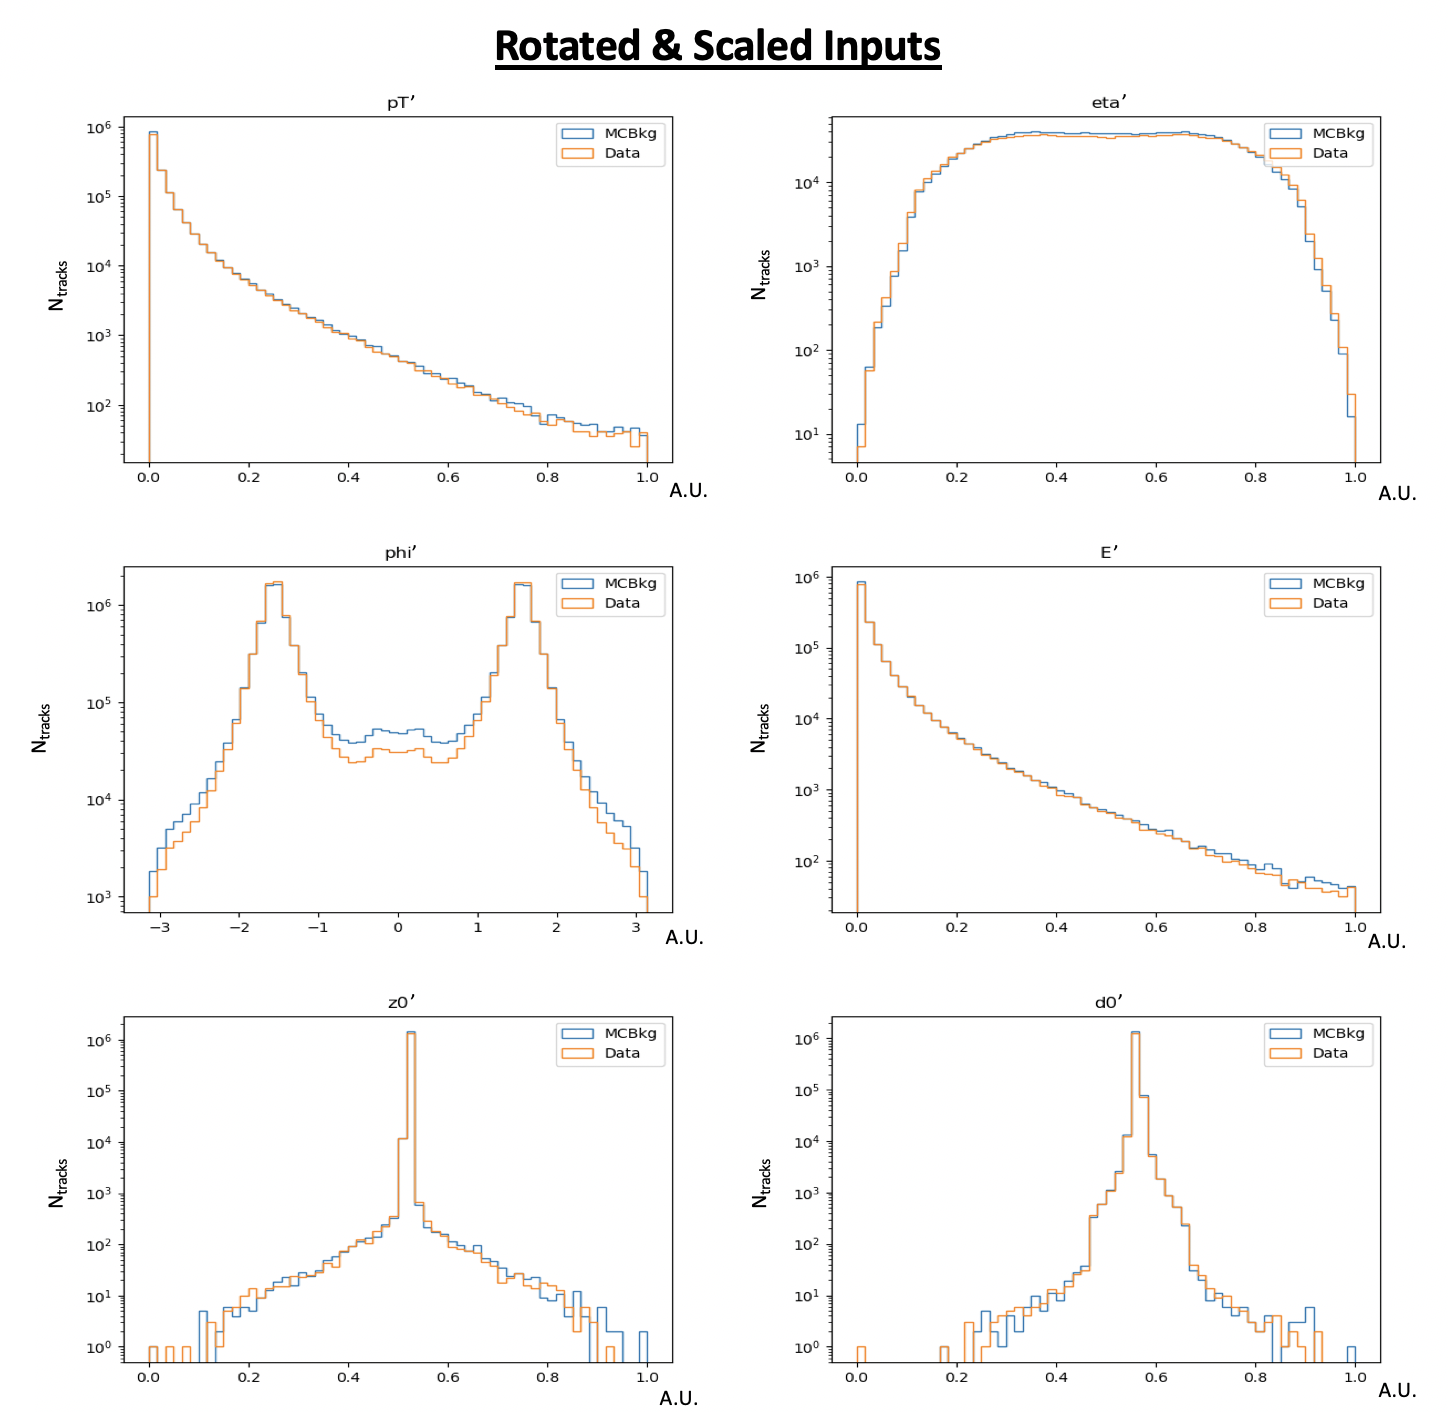
\includegraphics[width=0.7\textwidth]{figures/ml/pfn_datamc_input}
    \caption{The 6 PFN track variables in data and background MC, after the scaling and rotation procedure is applied. There is excellent modeling of the data by the MC within the track variables. The slight discrepancy in the phi distribution is due to the modeling of dead TileCal cells by the QCD MC, which will be discussed in Chapter~\ref{ch:analysis}. The level of discrepancy is determined to be within tolerance given that the final result with be data driven and the QCD model is used in the PFN training only.
    \label{fig:pfn_datamc_input}}
\end{figure}

%--------------------
\subsubsection{Training}
\label{sec:pfn_training}

As seen in Figure~\ref{fig:pfn_arch}, two separate architectures are defined and combined to do the supervised training. The PFN uses a masking layer to suppress any zero-padded inputs, making the architecture length agnostic. The masking layer ignores any all-zero inputs in the summation layer. Additionally, The summation layer in the PFN enforces permutation invariance, so the network is unordered. The $\Phi$ network has 3 dense layers of dimensionality 75 with \textsc{relu} activation, with 27.5k trainable parameters and an output $\Phi$ latent space dimension of 64. \par

The classifier $F$ network similarly has 3 dense layers with 75 nodes with \textsc{relu} activation, and a final softmax layer to determine the event-level classification with a categorical cross-entropy loss. The Adam optimizer is used with an initial learning rate of 0.001. \par

The PFN is trained in a fully supervised way using SVJ signal MC and QCD MC events. Although several SM processes are expected to contaminate the SR (see Chapter~\ref{ch:analysis}), QCD is the dominant background. Training against a QCD-only sample is determined to produced better results than training on a more complete background - when training with a background which represents samples that are more enriched in \met, the ability of the PFN to identify high \met signals is reduced. When training with a QCD-only background, there is greater contamination from \met enhanced backgrounds in the final SR - however the increased signal acceptance means that overall sensitivity is still higher with a QCD-only training. This can be seen in the comparison of output classifier distributions in Figure~\ref{fig:fn_MC_training_mixture}.

\begin{figure}[!htbp]
\centering
   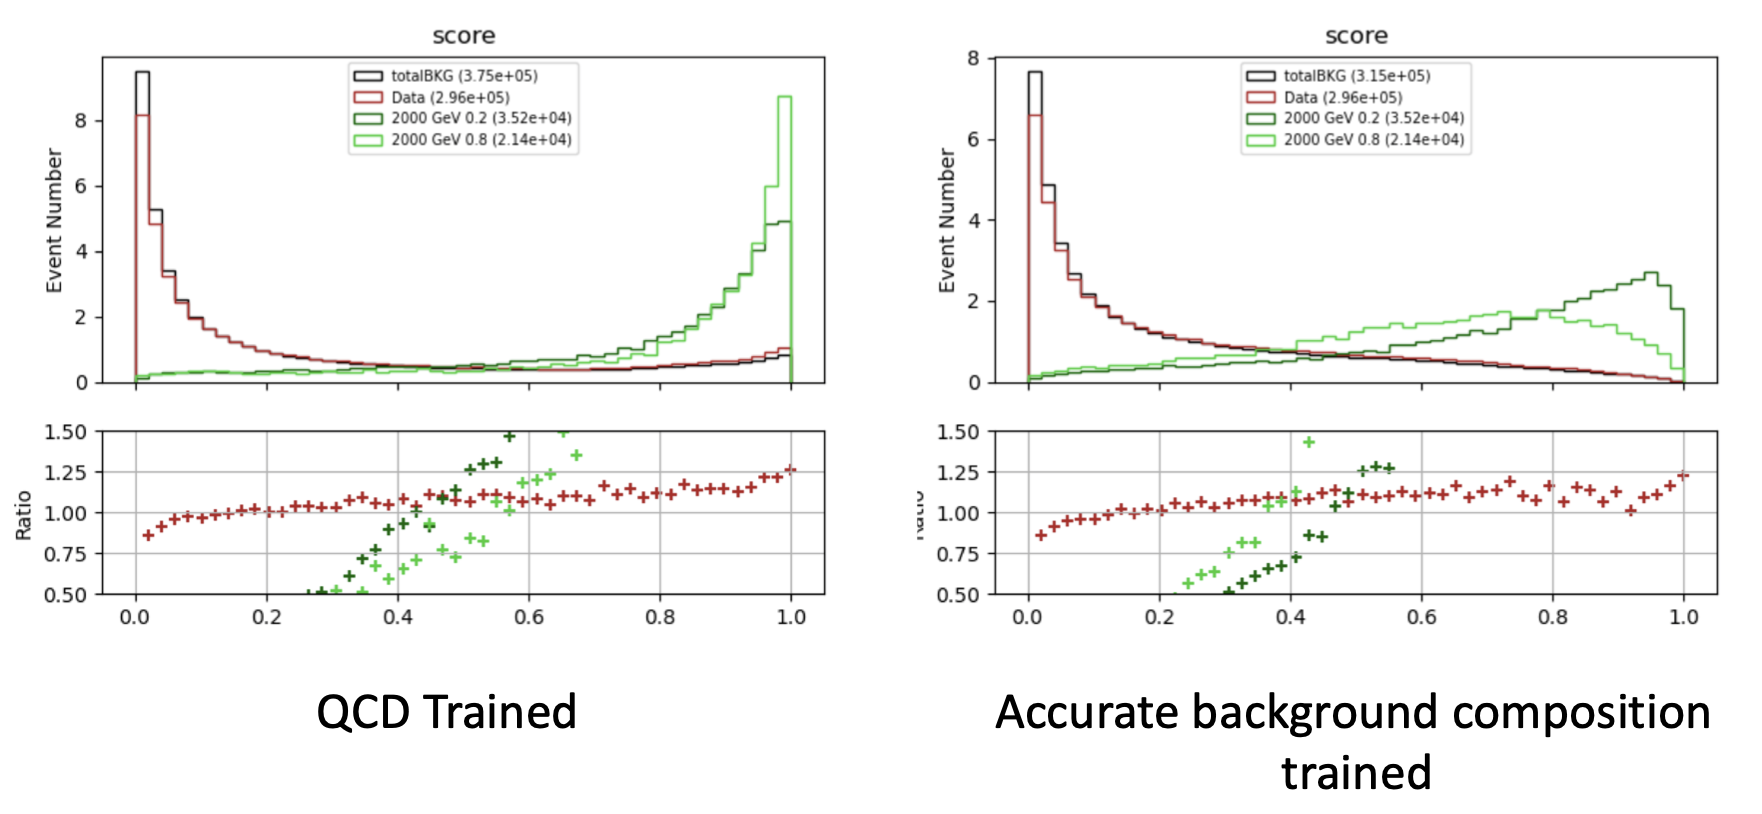
\includegraphics[width=0.9\textwidth]{figures/ml/pfn_MC_training_mixture}
    \caption{PFN score for background MC, data, and signal, comparing a PFN training on QCD-only vs all-background MC samples. The average AUC for the QCD-only training (left) is 0.93, while the average AUC for the mixed background training (right) is 0.84. The sensitivity estimate across the grid is better for the QCD-only training - from the distribution we can conclude that this is because the sensitivity to MET enhanced signals is greatly reduced.
    \label{fig:fn_MC_training_mixture}}
\end{figure}

500k events from both background and signal are used in training, where the signal is a combined file of all simulated signal points and the full QCD background which is sampled according to it's MC weights to produce the proper \pt~input shape. A study was done to check the optimality of the inclusive signal model PFN as compared to one trained on high and low \rinv~points separately, to better capture the differences in high and low~\met~ across signals and backgrounds, but a small effect is found and the decision is taken to keep the inclusive model (Appendix~\ref{app:pfn_qp}).\par

The network is trained for 100 epochs. A train/test/validation split of 78\%, 20\%, and 2\% is used for the final PFN training. Figure~\ref{fig:pfn_loss} shows the loss during training, which is stable and flattens by the end of training, and the final evaluated losses that provide signal-background discrimination over the test set.

\begin{figure}[!htbp]
\centering
   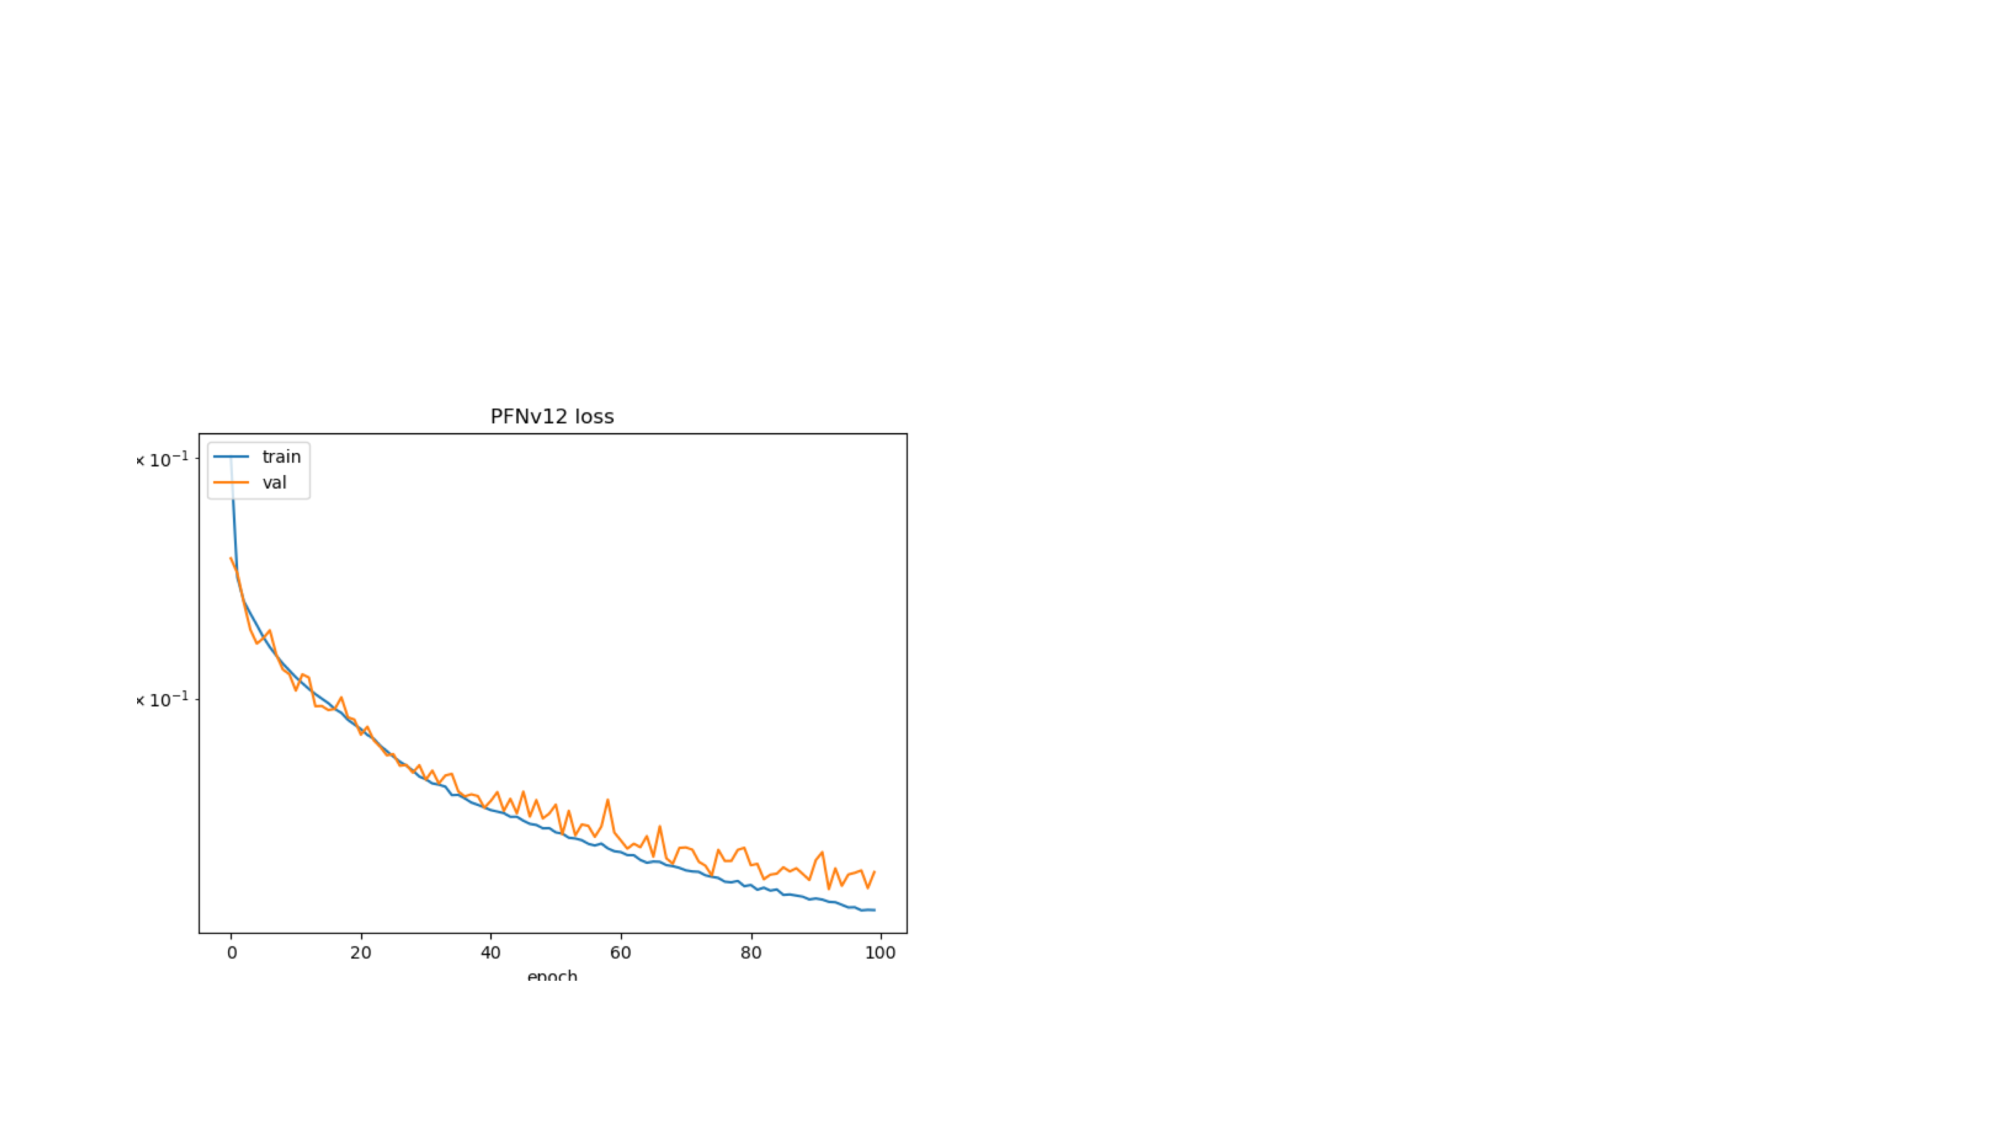
\includegraphics[width=0.45\textwidth]{figures/ml/pfn_loss}    
   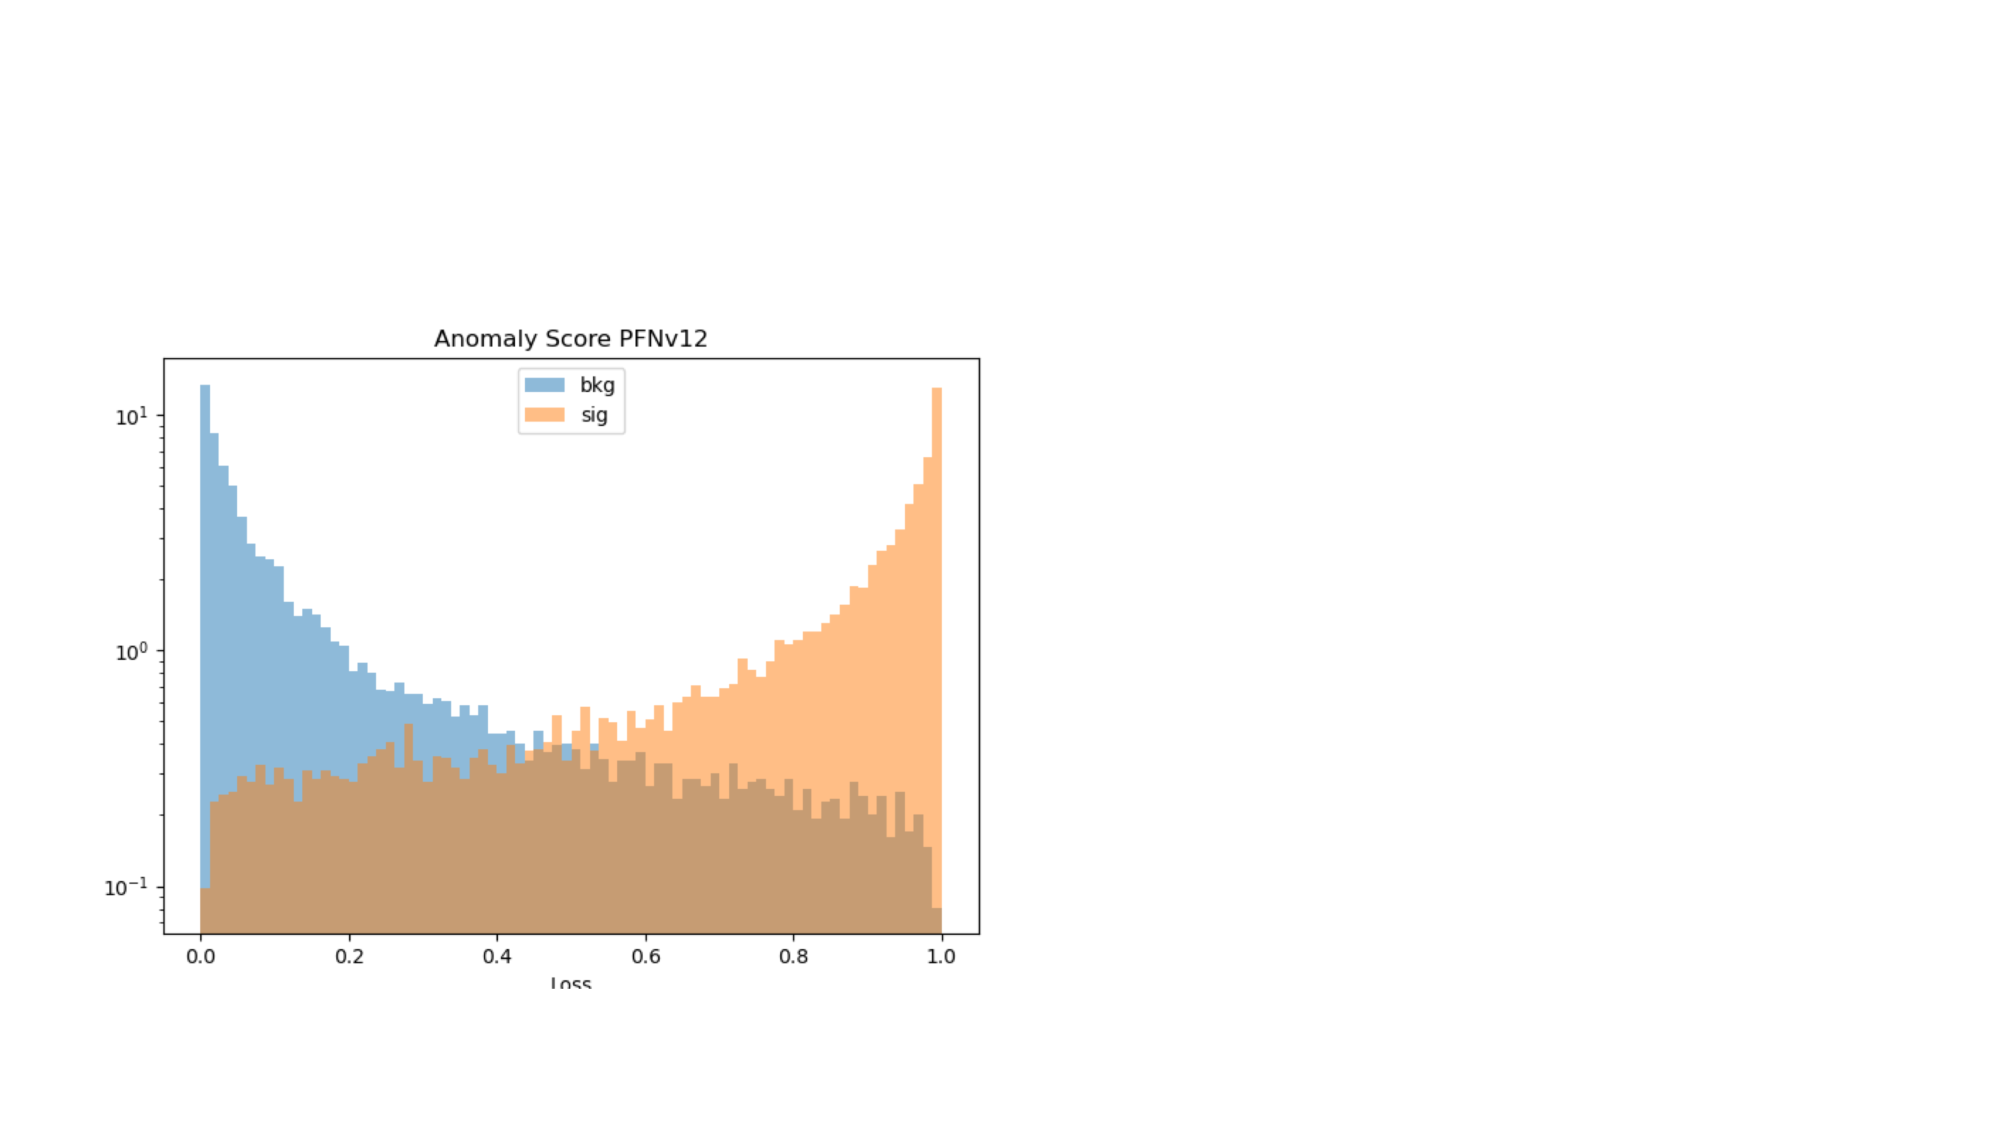
\includegraphics[width=0.45\textwidth]{figures/ml/pfn_score}    
    \caption{PFN architecture loss during training as a function of epoch (left) and the evaluated loss over the signal and background (right).
    \label{fig:pfn_loss}}
\end{figure}

Optimization studies were performed on the PFN, varying the number of training epochs, number of training events, batch size, learning rate, number of neurons, and dimension of the $\Phi$ space. A summary of these studies is presented in Appendix~\ref{app:pfn_qp}. The model presented here represents an optimal choice across these parameters.

%--------------------
\subsubsection{Performance}

The performance of the PFN can be assessed via the area-under-curve (AUC) of the receiver operating characteristic (ROC) associated to evaluating the PFN on the test set of signal and background events. Figure~\ref{fig:pfn_roc} shows the ROC curve of the PFN when classifying the QCD background from the combined signal, with an AUC of 0.93. Figure~\ref{fig:pfn_AUC_score_grid} shows the AUC of the PFN across the SVJ signal grid, demonstrating strong discrimination capability even in the varying corners of phase space. 
Figure~\ref{fig:pfn_score_all} shows the output score distribution in two signals, data, and the total background MC.
A selection of PFN score $>$ 0.6 for all SR events is chosen to maximize signal sensitivity across the grid. 
\begin{figure}[!htbp]
\centering
   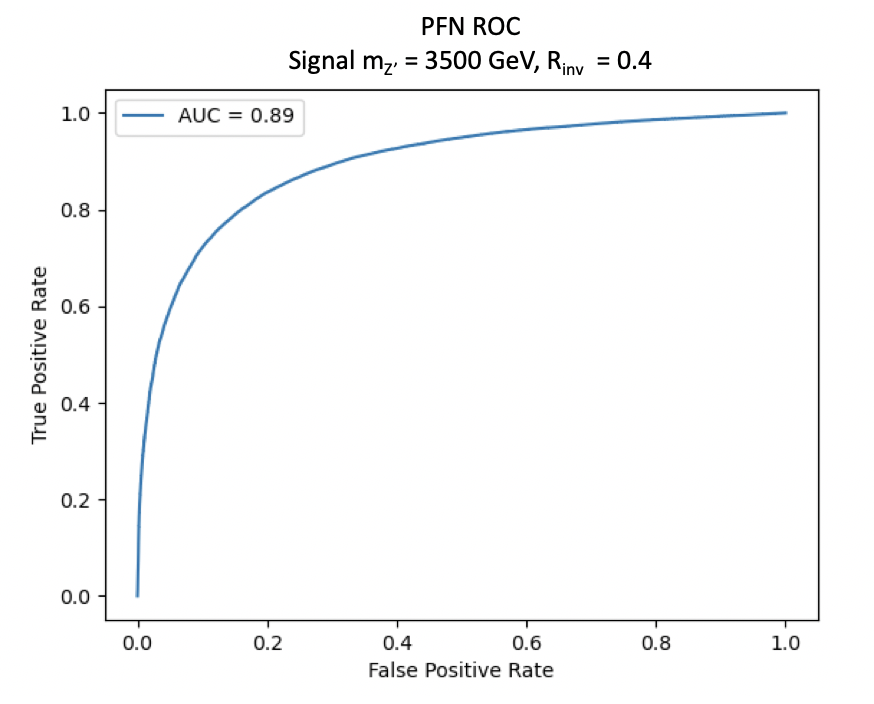
\includegraphics[width=0.7\textwidth]{figures/ml/pfn_roc}
    \caption{ROC the PFN score for combined signal (true positive) and QCD background (false positive).
    \label{fig:pfn_roc}}
\end{figure}
\begin{figure}[!htbp]
\centering
   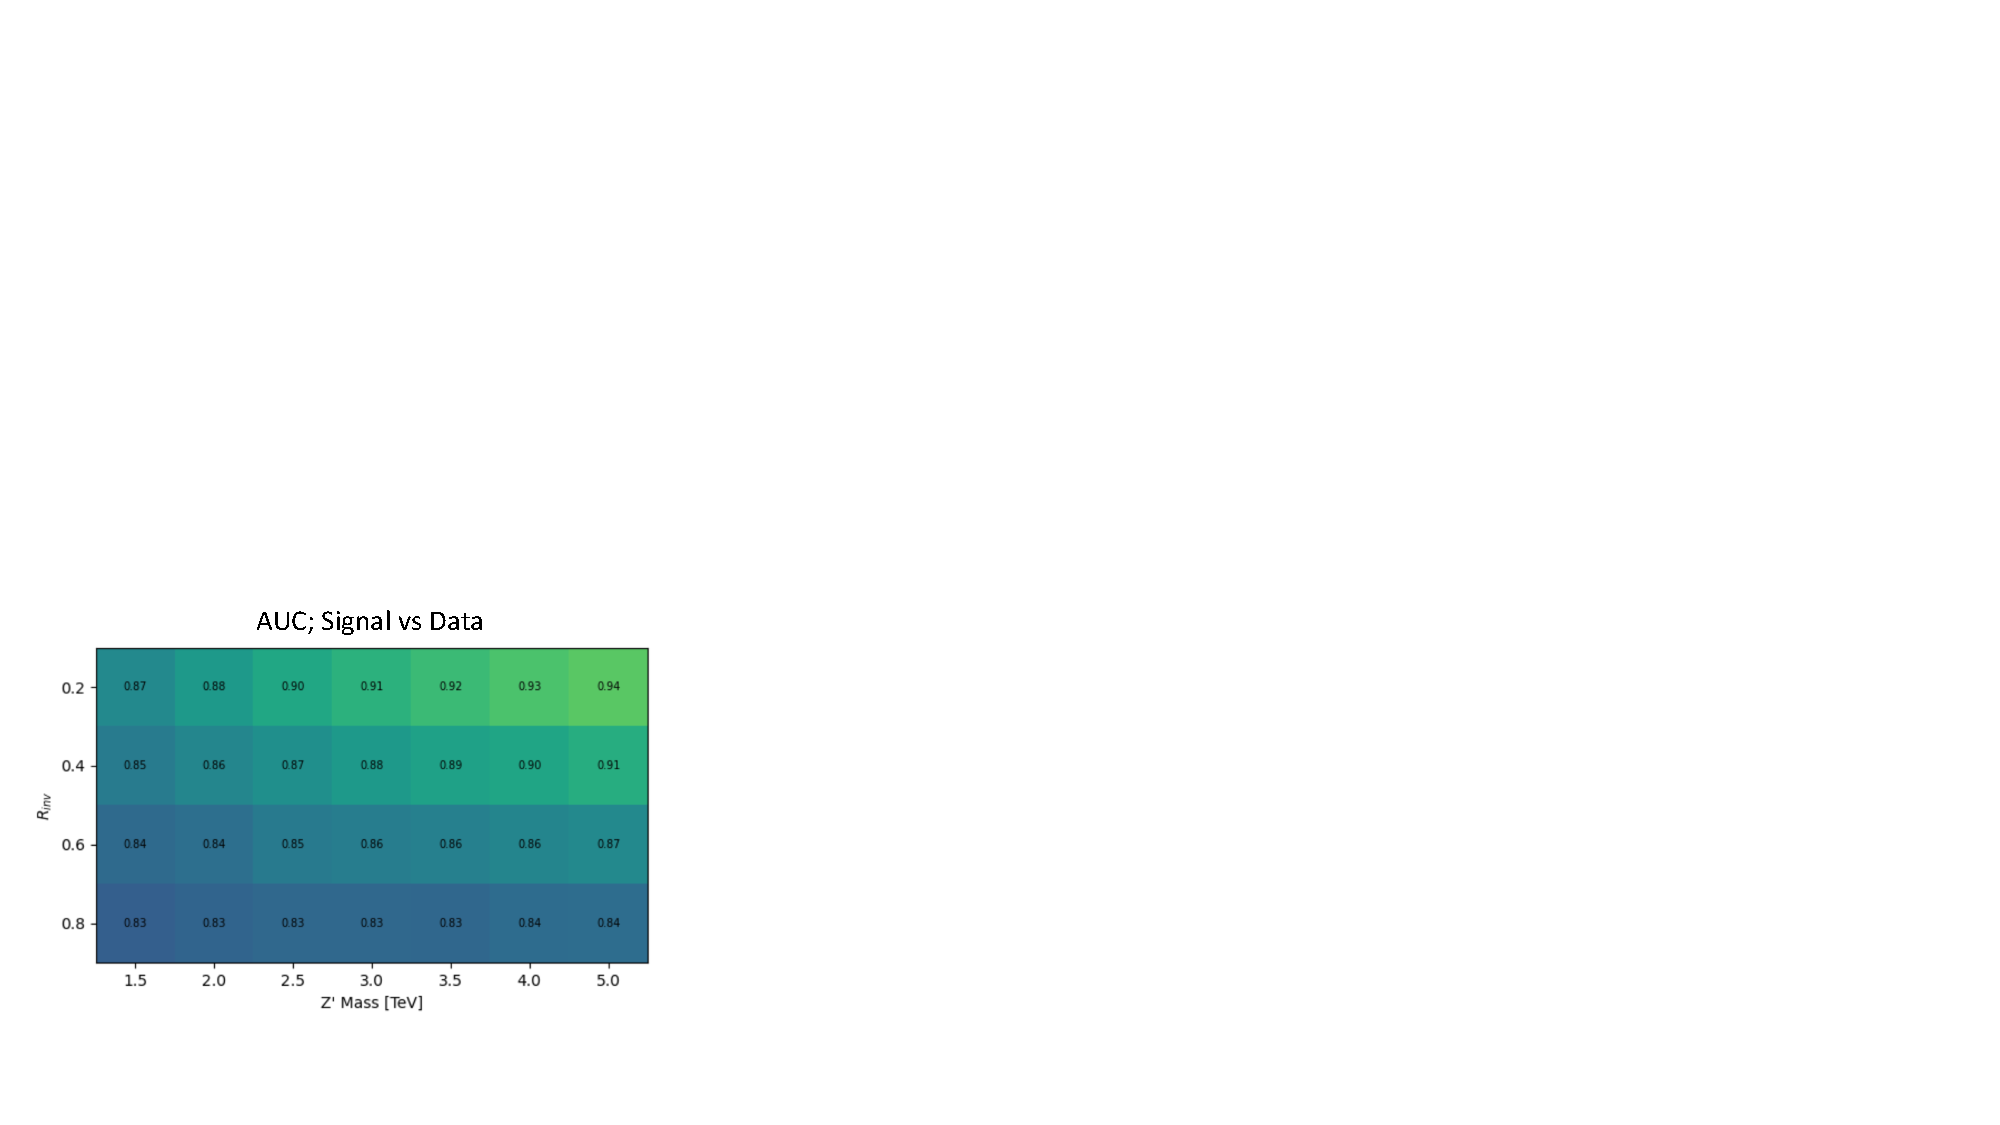
\includegraphics[width=0.7\textwidth]{figures/ml/pfn_AUC_grid}
    \caption{AUC from the PFN score for each signal in the SVJ grid, shown versus the QCD-only training sample.
    \label{fig:pfn_AUC_score_grid}}
\end{figure}


\begin{figure}[!htbp]
\centering
   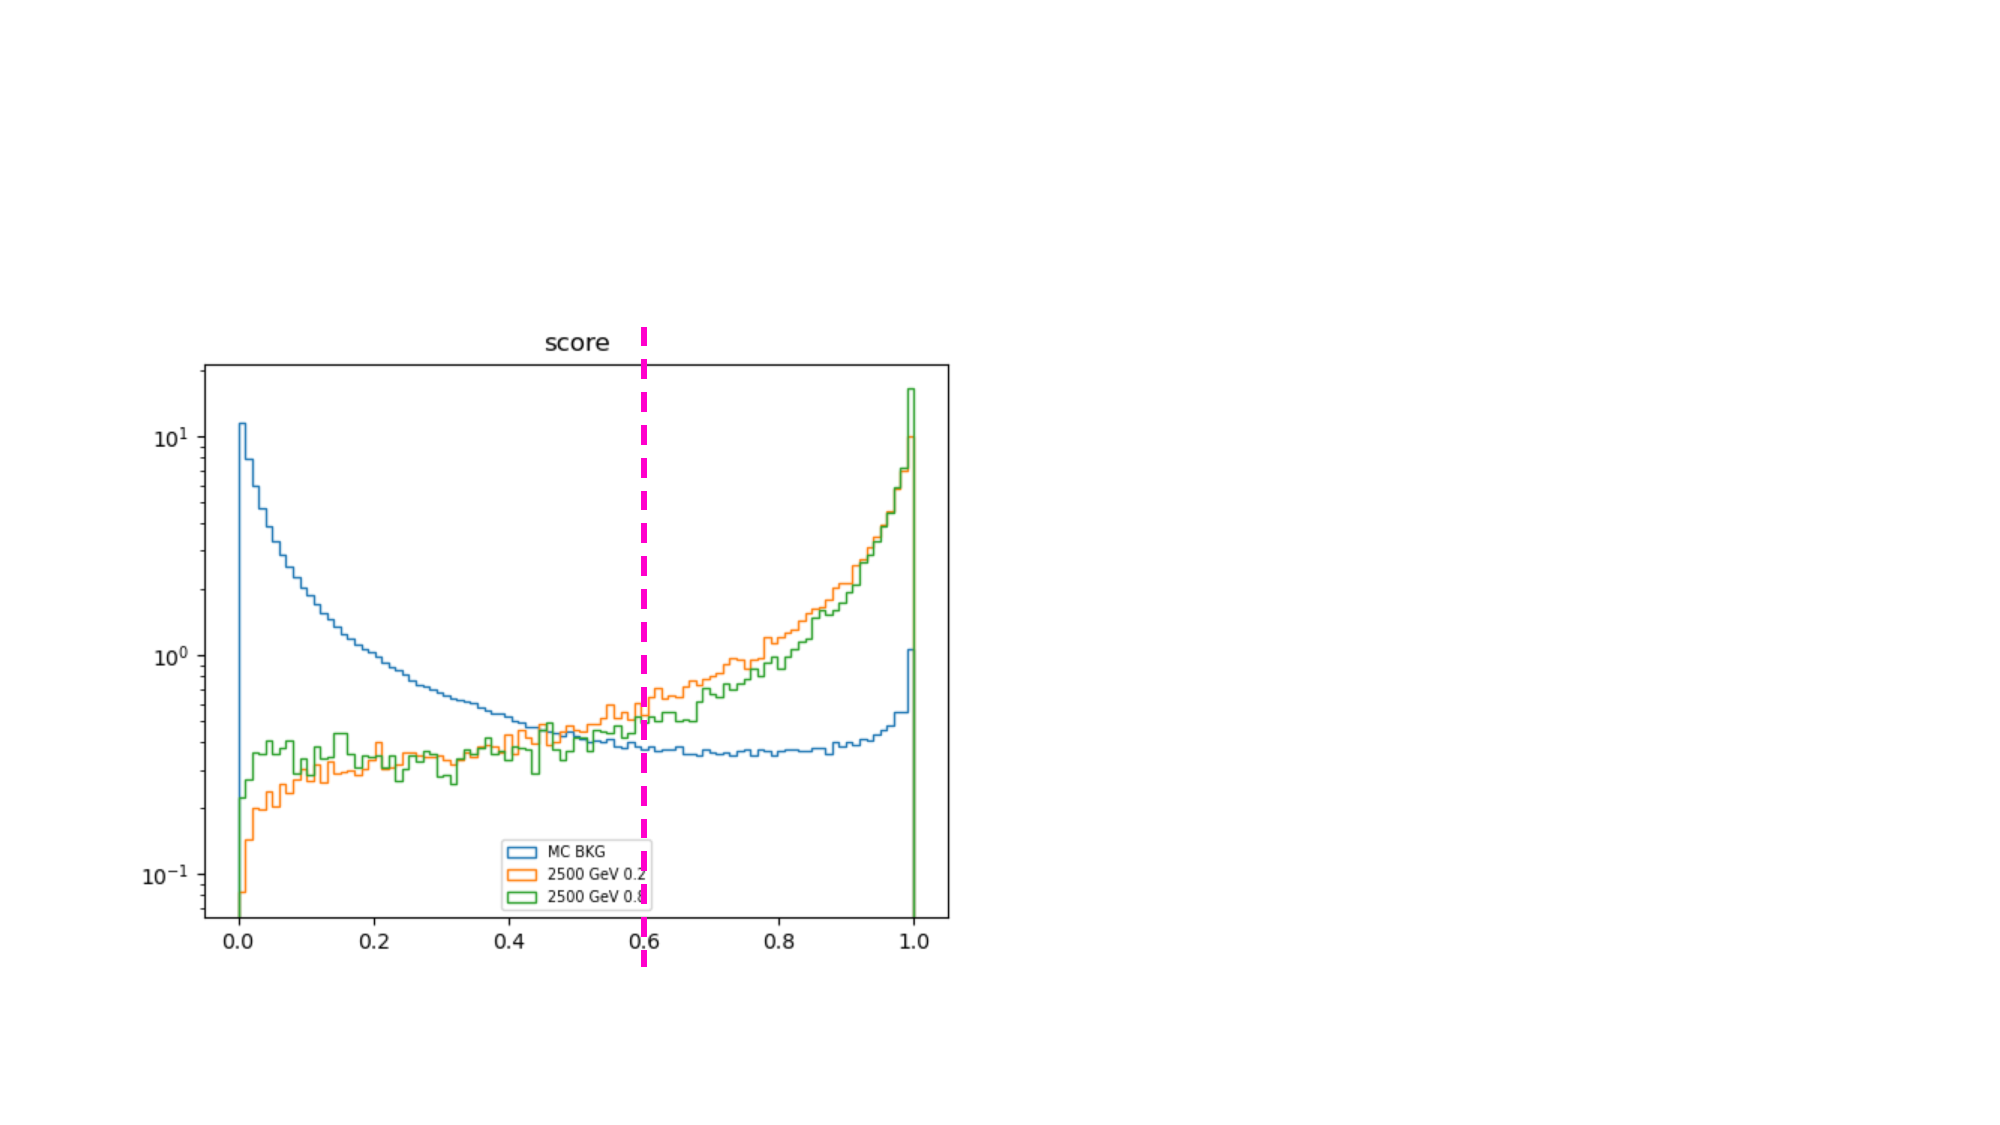
\includegraphics[width=0.45\textwidth]{figures/ml/pfn_score_all}
   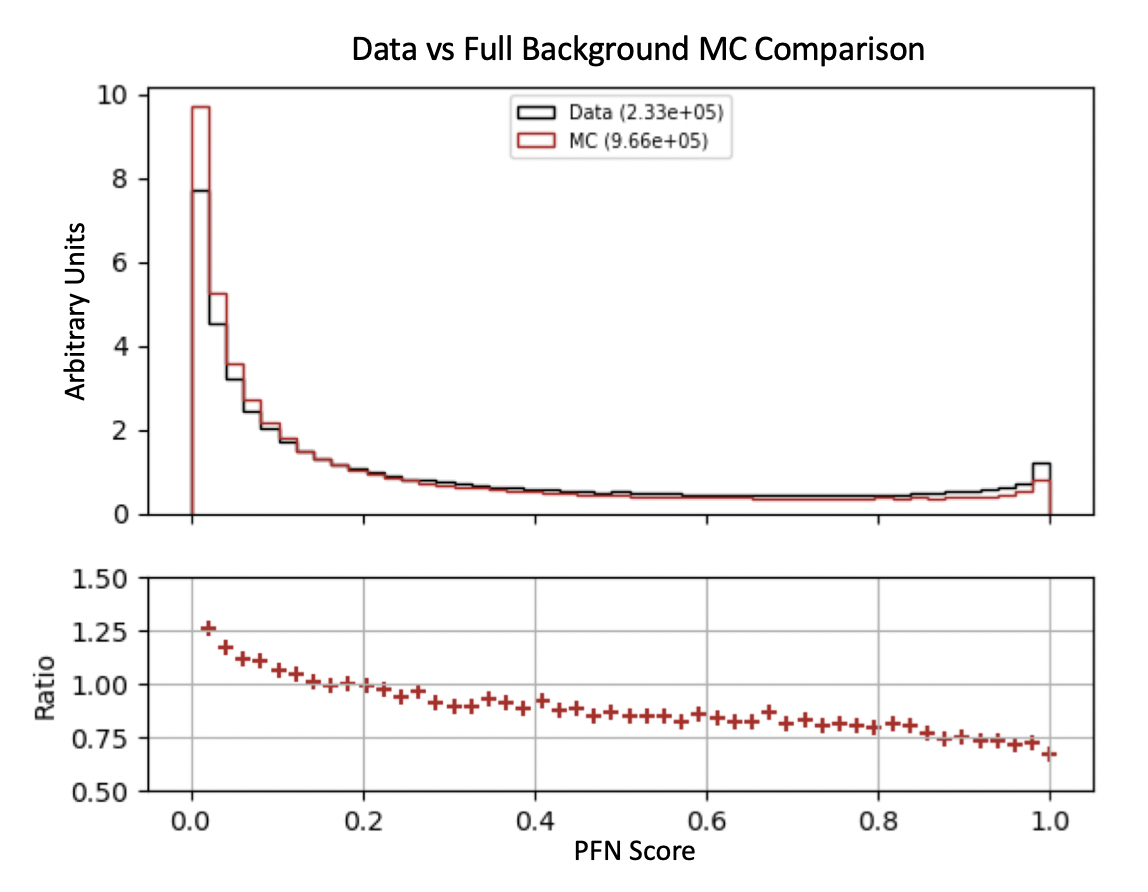
\includegraphics[width=0.45\textwidth]{figures/ml/mlscore_effComp}
    \caption{PFN score for two signals and the total background MC (top), and between data and MC (bottom). The difference between data and MC efficiency is minimal ($<$ 5\%).
    \label{fig:pfn_score_all}}
\end{figure}

Another supervised approach was studied using a BDT as the primary selection tool, trained over high-level variables describing each event. 
Studies comparing the PFN and BDT approaches are provided in Appendix~\ref{app:bdtvspfn}.
Ultimately the low-level high-dimensional approach offered by the PFN was selected for its increased performance and lessened kinematic dependence.

Appendix~\ref{app:ml} shows more studies on the ML methods and comparisons of varying approaches. 

\clearpage

